\chapter{绪论}\label{chap:introduction}

\section{选题的背景及意义}
%% 问题定义与介绍
光照估计(又称光照分布估计)是从已知的彩色图像信息中,预测、估计、恢复出整个场景的光照分布。该问题的输入通常是若干张彩色图片,或者是一段视频,有时已知的几何或材质信息也被用来辅助估计光照。场景的光照分布是指场景中各个方向的光照的颜色和强度。较为常见的光照分布表示方法包括高动态范围(High Dynamic Range,HDR)全景图、球形谐波(Spherical Harmoins,SH)函数表示、基于物理的Sun-Sky模型表示等。
其中精度最高、使用比较广泛的是HDR全景图像,而在实时渲染领域使用较多的是光照的SH表示。 基于物理的光照模型则多用于室外场景。

%% 研究意义、应用场景
光照估计作为计算机图形学和计算机视觉的基础问题之一,有着广泛的实际应用场景。例如:基于图像的渲染(Image Based Rendering,IBR)、增强现实(Augmented Reality,AR)、电影后期制作、真实感虚实交互等。图\ref{fig:demo-problem-define}展示了光照估计的应用之一。光照估计也与这两个学科中的许多其它问题息息相关。例如:双向反射分布函数(BRDF)估计、场景几何重构、本征信息提取、图像增强,等等。高质量的光照估计结果通常能够为这些问题的解决带来很大的帮助。\begin{figure}[!htbp]
    \centering
    
\includegraphics[width=0.40\textwidth]{Img/ucas_logo.pdf}

    \bicaption[光照估计的应用]
    {光照估计的应用之一。使用单张图片估计场景的光照,并利用估计的光照渲染一个新的物体合成到图像中。
    可以看出使用估计光照渲染后的3D物体,与场景中的已有物体在视觉上较为一致。}
    {3D rendering under the predicted illumination.
    visual effect of the 3D rendering is in line with the original image.}
    
    \label{fig:demo-problem-define}
\end{figure} 

%% 难点
从有限的图像信息估计出整个场景的光照分布是一个复杂的问题。首先,图像的视野范围比较有限,例如一张视场角(FOV)为60°的照片所拍摄到的区域,在其对应的全景图中占比不足6\%。此外,一幅图片是光照分布、场景几何结构、物体材质、摄相机参数等多个单位之间的复杂交互结果(公式~\ref{eq:complex-interaction-result})。
\begin{equation} \centering 
    \label{eq:complex-interaction-result}
    Image = ComplexInteraction(Light, Geometry, Material, Camera)
\end{equation}
通过公式\ref{eq:complex-interaction-result}可以看出,在其它三个信息未知的情况下,从图像(Image)反推出光照(Light)是一个严重的不适定(ill-posed)问题。不仅如此,在不同的条件下拍摄的彩色图像可能存在很多误差。例如图像中的过曝光/欠曝光区域、相机畸变、不正确的白平衡等。这些都会对光照估计造成一定程度的干扰,增加光照估计的难度。

%% 传统方法 + 局限性
为了简化问题难度,传统方法常常增加输入信息的数量或缩小光照模型的规模。其中一部分工作使用更多的输入信息辅助估计场景光照。例如深度信息、几何信息、多张图片、先验知识、用户标记等等。这类方法或依赖特殊的探针、或依赖特殊的拍摄设备、或依赖额外的辅助信息与模型假设,均具有一定的局限性。另一部分工作通过使用低维的光照表示模型来简化光照估计问题,例如使用球形谐波函数(SH)来拟合场景光照、使用小波函数近似场景光照、使用若干个点光源的集合近似场景光照、使用基于物理的室外光照模型等等。可以看出,无论是增加输入信息还是使用简化的光照估计模型,传统光照估计方法都具有很大的局限性。

%% 深度学习方法 + 局限性
近年来,深度学习在多种计算机视觉问题上大放异彩,用于分割、检测、标识、分类的神经网络层出不穷。一些研究者尝试将深度学习应用在光照估计问题当中。其中Hold-Geoffroy等人\cite{hold2017deep}和Gardner\cite{gardner2017learning}等人的工作是应用深度学习估计光照的最先进方法。它们在大规模数据集上训练了一个深度卷积神经网络,分别用于室内和室外的场景光照估计,能达到较好的效果。不过,目前已有的深度学习方法也有一定的局限性。训练一个鲁棒的神经网络往往需要大量的数据,而目前用于光照估计问题的数据集比较有限,主要包括:大规模的低动态范围全景数据集(SUN360\cite{xiao2012recognizing}等)和中小规模特定场景的高动态范围全景数据集(Laval Indoor等\cite{gardner2017learning})。这些数据集在规模和质量上很难同时到达训练深度神经网络的要求。

%% 研究目标和研究方法, 在前人工作的基础上,对网络、loss、优化,数据 展开研究
在这样的背景下,本文在光照估计的两个方向开展研究。其一是构建一个具有一定规模和质量光照估计的数据集。这样的数据集不仅能被用来训练更加鲁棒的光照估计网络,也可以被应用到其它多种相关的深度学习问题当中。其二是在已有数据集和本文构建的数据集基础上,深入探索基于深度学习的光照估计方法,对其中的网络结构,网络参数,损失函数,光照表示等多个模块进行细致的对比和研究。

\section{国内外研究现状}
\subsection{光照的表示}
光照的表示对光照估计问题至关重要。场景的光照分布有着多种多样的表示方法。其中高动态范围(High Dynamic Range,简称HDR)全景图是一种被广泛使用而且精度较高的光照表示方式。与普通的8位三通道图像不同,HDR图像的颜色值范围可以从0取到非常大。这意味着HDR图像可以更细致地表示每个像素位置的真实亮度值。因此无论是HDR全景图表示的光照,还是使用其渲染的物体,都能更接近真实值。Reinhard等人在\textit{High Dynamic Range Imaging}\cite{reinhard2005high}中对HDR图像进行了详细的介绍。

%%HDR全景图表示的光照在图像渲染、估计光照等问题中往往比较“繁琐”。
研究者们也提出了一些小巧、高效的光照近似模型,代价是牺牲一部分精度。Ramamoorthi和Hanrahan\cite{ramamoorthi2001efficient}提出使用球形谐波函数来表示场景的光照。这种方法表示的光照,不仅参数规模较小,而且其在渲染物体时非常高效。他在文章中指出,该模型仅使用9个系数时,在漫反射物体上渲染结果的平均误差也不超过1\%。不过由于球形谐波函数本身的特性,这种方式不能很好的保留光照分布的高频细节。尽管如此,它的简洁和高效使得它成为实时渲染中的重要方式之一\cite{green2003spherical,sloan2008stupid}。许多光照估计方法中采用了这种模型来表示场景的光照分布。图\ref{fig:lighting-representation}展示了不同的几种光照表示示例。\begin{figure}[!htbp]
    \centering
    
\includegraphics[width=0.40\textwidth]{Img/ucas_logo.pdf}

    \bicaption
    {几种不同的光照表示模型对比}
    {Comparison of different representations of illumination}
    
    \label{fig:lighting-representation}
\end{figure}

在室外场景中,光线的主要来源是太阳光、太阳光在空气中的散射折射、以及光在地面的反射。因此基于物理的光照表示模型更加适合表示室外场景。Perez等人\cite{perez1993all}提出一个参数化的物理模型来表示天空中的发光度(Luminance)分布。
之后的许多工作~\cite{nishita1996display, sirai1993display, preetham1999practical,raab2008unbiased}考虑了空气散射和折射、大气浑浊度的影响,将该模型扩展为多种不同类型颜色模型。Hosek和Wilkie\cite{hosek2012analytic, hovsekhovsek2013adding}基于这些工作,考虑并加入了多种因素,整理出一个可调节太阳位置、大气浑浊度、地面反照率的物理参数模型。这类模型的参数量较小,精度也很可观,因此成为室外场景光照估计问题中常用的光照表示方法。

光照分布也有很多其它的表示方式。Ng等人\cite{ng2003all}提出使用小波函数来近似光照分布。LeGendre等人\cite{legendre2016practical}提出了一个实用的框架,能够使用LED灯台精确地重构出各个方向的场景光照。近期Weber\cite{weber2018learning}结合深度学习,使用自编码器(auto-encoder)对光照分布进行建模,为光照估计问题提供了新的思路。

\subsection{使用光探测物估计光照} 
光照估计是一个复杂的问题,研究者们常常采用多种方法的组合来解决这个问题。使用光探测物(light probe)来估计光照就是这些方法之一。常见的光照探测物包括:镜面球体,漫反射球体,镜面反射/漫反射混合球体,人眼,人脸等等。Debevec\cite{debevec1998rendering}建立了一个基于光照模型的虚拟物体插入系统。其中所涉及光照的就是使用镜面反射球体作为光探测物来估计的。该工作首次提出可以通过拍摄不同曝光下的镜面球体,来获取一张高动态范围的全景图片。在之后的工作中,Reinhard等人\cite{reinhard2005high}和Debevec等人\cite{debevec2012single}指出,使用一个漫反射球体,或者漫反射与镜面反射表面混合的球体,也可以达到同样的效果。 值得一提的是,Debevec在其工作\cite{debevec1998rendering}中,将远距离场景、近距离场景、以及待插入的虚拟物体分离开,并假设插入的虚拟物体并不会造成远距离场景的变化。之后的虚拟物体插入、增强现实等工作都遵从了这个假设。
\begin{figure}[!htbp]
    \centering
    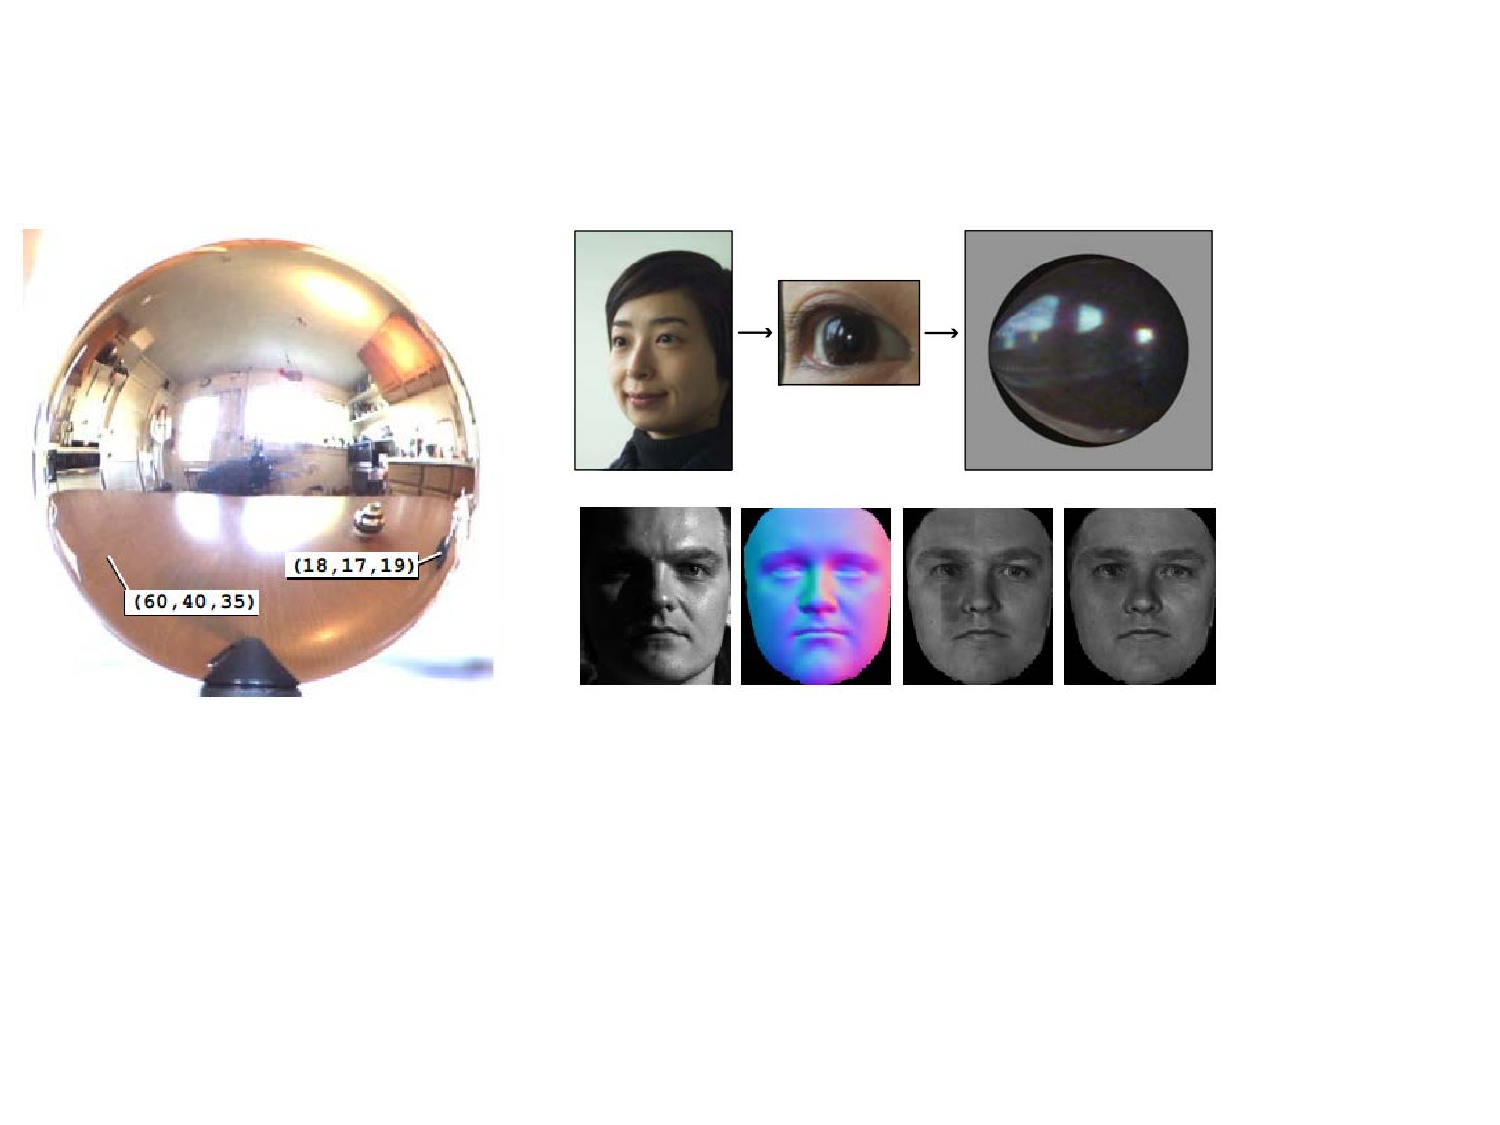
\includegraphics[width=1.0\textwidth]{Img/light-probe.pdf}

    \caption[几种用于光照估计的光探测物]
    {用于光照估计的光探测物——球\cite{debevec1998rendering}、人眼\cite{nishino2004eyes}、人脸\cite{wang2007face}}
        
    \label{fig:light-probe}
\end{figure}
上述的光探测物大多是已知物体几何和表面材质、且预先放置在场景中的规则物体。还有一些特殊的“物体”也可以作为光探测物。例如人的眼球,人脸,人手等常出现照片中的元素。Tsumra等人\cite{tsumura2003estimating}在假设人眼是规则球体的前提下,利用眼球上光线的反射,估计场景的光照。Nishino和Nayar\cite{nishino2004eyes}分析了眼球的大致结构,并利用包含眼球的照片估计场景的光照分布。不过该方法需要分辨率和清晰度较高的相机,而且其文中也指出该方法没有考虑瞳孔颜色、虹膜颜色等因素。而这些因素都会对光照估计产生较大影响。人脸作为照片中经常出现的物体,也经常被用作光探测物。
Wen等人\cite{wen2003face}通过一张人脸照片,估计出光照的SH表示进而对人脸实现重照(relight)。Wang等人\cite{wang2007face}提出来一种基于马尔科夫随机场的能量最小化框架,意图从正脸照片中恢复出人脸的形状、反照率和光照。   
在之后的工作中Shim\cite{shim2012faces}、Knorr等人\cite{knorr2014real}、Shahlaei和Blanz\cite{shahlaei2015realistic}探索了如何从人脸照片中估计较为精确的光照。Yao等人\cite{yao2013hand}使用普通相机和深度相机下的人体手部图像,通过人手的亮度和法线,估计出由若干个球形谐波系数近似的低频光照。

可以看出,这类估计光照的方法都需要一个已知其类型、几何、材质的光探测物存在于场景内,图\ref{fig:light-probe}展示了常见的光探测物。无论是规则的球体,还是人的各个部位,它们都需要照片中包含指定的物体和元素。而在大多数的光照估计问题中,很难保证这些标志物或探测物一定存在,这无疑限制了此类方法的应用。

\subsection{使用特定设备估计光照}
\begin{figure}[!htbp]
    \centering
    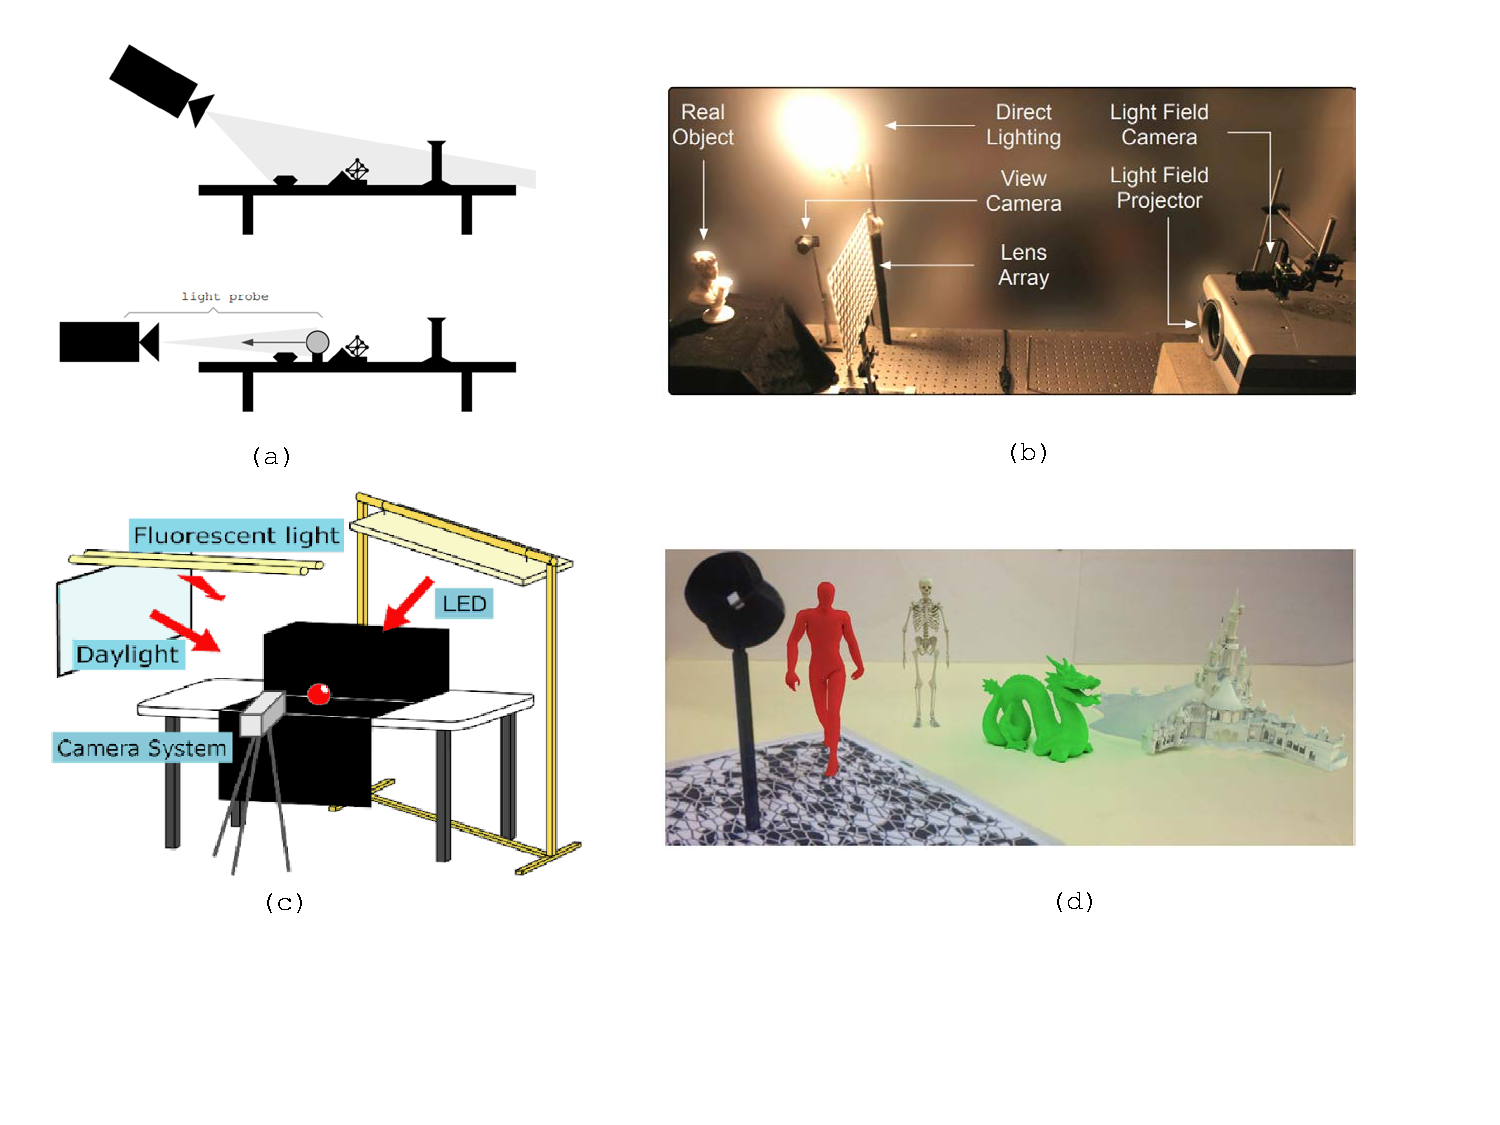
\includegraphics[width=1.0\textwidth]{Img/estimation-using-devices.pdf}

    \caption[使用特殊设备估计光照]
    {几种使用特殊设备估计场景光照的系统:(a)Debevec\cite{debevec1998rendering}通过多次拍摄获取光照的示意图;(b)Cossairt等人\cite{cossairt2008light}的复杂拍摄系统;(c)Imai等人\cite{imai2011estimation}使用的拍摄设备;(d)Cailian等人\cite{calian2013shading}用于AR光照估计的设备示意图。}
    %%{Illumination estimation system using specific devices.}
    
    \label{fig:estimation-using-devices}
\end{figure}
降低光照估计问题难度的另一个思路是使用特定的设备、装置或应用辅助估计光照。Pilet等人\cite{pilet2006all}使用多个不同位置的相机和一个平面标定物构建了一个3D估计系统。通过追踪该平面标定物并计算其中的高光和阴影,估计出场景中的几何和光照。Yoo和Lee\cite{yoo2008real}提出了一个由鱼眼镜头、中性衰减片(Neural Density Filter,ND)和普通相机构成的光照探测系统。他们通过鱼眼镜头获取一个半球面,使用ND片直接感知明亮区域,并通过一系列算法实时地估计场景中的光照。Cossairt等人\cite{cossairt2008light}使用一组透镜、光场相机、光场映射器,构建了一个适合单光源较暗场景下的光照估计系统。随后Imai等人\cite{imai2011estimation}使用多光谱成像设备,探究了可变亮度阈值、色调、偏振滤镜在检测光照条件较为复杂的场景下的高光分布。提出了适用于偏高光反射物体上的光照估计方法。Tocci等人\cite{tocci2011versatile}构建了一个光学设备,用以获取影视级别的高动态范围视频。Manakov等人\cite{manakov2013reconfigurable}提供了一个插件类型的相机硬件,用以与高动态范围图像,多光谱、偏振和光场等相关的应用。Cailian等人\cite{calian2013shading}使用一个阴影探测器,来解决实时增强现实中的光照估计问题。K\'an和Peter\cite{kan2015interactive}通过全景图像拼接技术,建立了一个在智能相机中用于捕捉高动态范围全景图的应用。
不过,通过这些使用特殊设备或者特定应用获取场景光照的方法并不是严格意义上的光照估计。他们其实是倾向于解决快速获取高动态范围图像或视频的工程问题。图\ref{fig:estimation-using-devices}展示了上述的一些的光照估计系统的使用情景,可以看出,这种光照估计方法所需的设备通常比较复杂。虽然在实验室环境中能够有效运行,但是这些设备的类型和数量无疑提高了这种方法的应用门槛。

\subsection{使用额外信息估计光照}
从单张图片恢复或估计出整个场景的光照分布是个复杂的问题。借用额外的信息是光照估计问题中最常用的方法。借助的信息包括深度图像信息、场景几何形状、物体几何结构等等

深度信息对于光照估计问题有着很大的帮助。Knecht等人\cite{knecht2012reciprocal}借助深度相机和鱼眼镜头重建场景模型并提取了光源位置。Meilland等人\cite{meilland20133d}利用深度相机实时地创建稠密的高动态范围全景图,并使用K-means 算法从环境贴图中提取点光源位置。 Barron和Mailk\cite{barron2013intrinsic}提出了一种从彩色图像和深度图像中提取本征信息的方法。他们使用具有噪声的深度图像来辅助估计场景的几何结构,并在这些信息的基础上进一步提取彩色图像中的本征信息。Zhang等人\cite{zhang2016emptying}使用RGBD相机,将拍摄到的室内场景建模为一个包含光源、材质和几何的没有杂物的房间模型。并提供了对该模型进行场景编辑的方法。

\begin{figure}[!htbp]
    \centering
    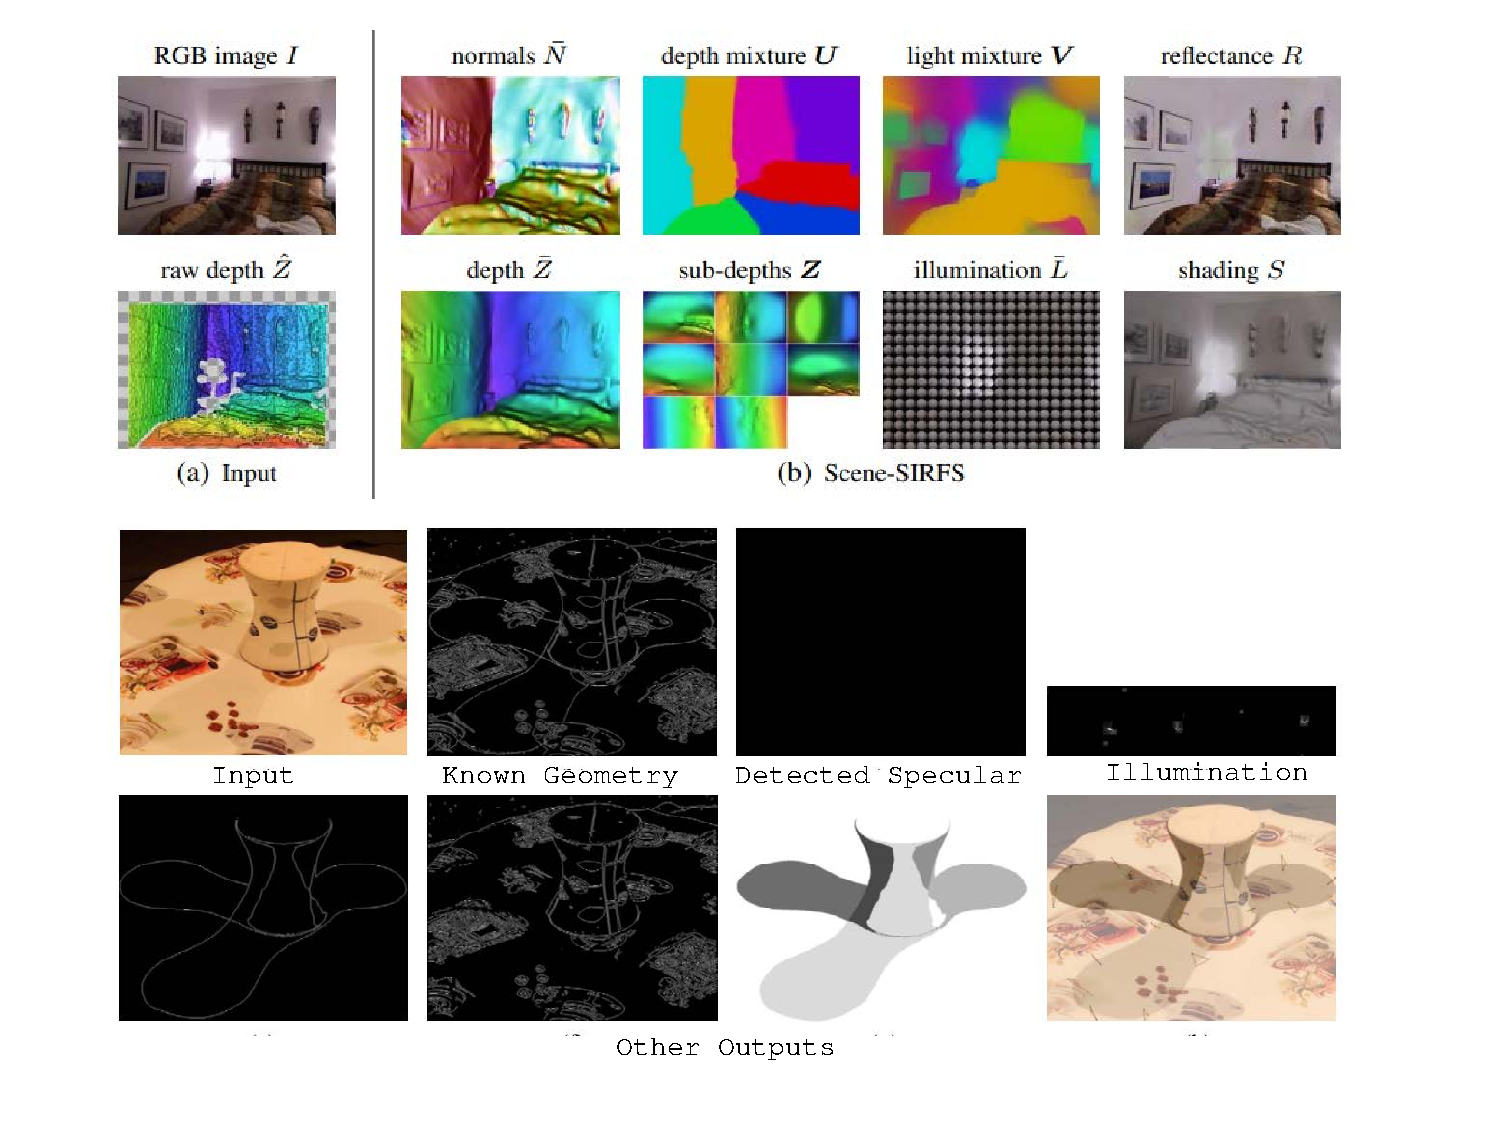
\includegraphics[width=1.0\textwidth]{Img/additional-input.pdf}

    \caption[使用额外信息辅助估计光照的方法]
    {借助深度信息和几何信息估计场景中的光照分布。上图是Barron和Mailk\cite{barron2013intrinsic}使用Depth信息作为额外的信息估计光照。下图则是Li等人\cite{li2003multiple}使用额外的几何信息作为额外信息估计光照。}
        
    \label{fig:additional-input}
\end{figure}
在已知场景几何或物体几何结构的情况下估计场景光照的分布也是主要的研究方向之一。例如,在表面形状类似桌子、平台、平板等结构的场景中,Li等人\cite{li2003multiple}的方法可以结合图片中的阴影、明暗、高光信息估计出多个方向的光源信息。Ramamoorthi和Hanrahan\cite{ramamoorthi2001signal}使用物体的几何结构和多个视角下的照片作为输入,估计出照片中物体的表面材质并进一步计算所在场景的静态光照信息。不过该方法需要多种假设——曲线表面、各向同性BRDF、没有多重反射等。Sato等人\cite{sato2003illumination}指出通过物体遮挡关系估计场景光照的有效性。他们通过分析给定几何的物体上的明亮区域和阴影区域,估计出较为真实的场景光照。在给定朗伯体(Lambertian)反射的物体几何时,Wang和Samaras\cite{wang2002estimation}的方法可以从单张图片估计出多个方向的光照信息。Panagopoulos等人\cite{panagopoulos2011illumination}提出了一个新的框架,来从单幅图片和粗糙的3D几何中,恢复出光照环境和估计场景中的投影阴影。该方法描述了一个高阶马尔可夫随机场(MRF)照明模型。该模型将低阶阴影证据与高阶先验知识相结合,用于投影阴影和照明环境的联合估计。

此外还有一些方法在已知物体类型的情况下,利用图片中物体的先验或者假设知识来帮助估计光照。例如前文提到的Nishino和Nayar\cite{nishino2004eyes}假设人的眼球是规则的球体,并基于此假设从人眼估计场景的光照。类似的方法\cite{barron2015shape, lopez2010compositing}虽然不需要预先知道精确的场景几何结构,但都要通过图像中物体的类型得到一些先验知识、假设和约束。进而分析、预测、估计、恢复出场景光照。

%% 多张图片
增加彩色图片的数量也会对光照估计有很大帮助。Sato等人\cite{sato1999acquiring}使用两张全方位全角度的照片构建出场景的大致几何,然后根据用不同快门速度拍摄的全方向图像序列计算场景的辐射度,并将其映射到构建的几何模型上。这个映射到几何上的辐照度分布就可以作为光照来渲染新的3D物体。Nishino等人\cite{nishino2001determining, nishino2005re}在已知物体的大致几何的情况下,分别为发光体和普通物体拍摄多张图片来估计场景的光照。Yu等人\cite{yu2006sparse}则通过多视角图片来恢复出固定光照条件下的物体纹理和光照分布。Wu等人\cite{wu2011high}建立了一个纯基于图片的形状、表面、光照的估计模型。Shan等人\cite{shan2013visual}在解决重构场景的问题时,提出了一种从大规模不同光照条件图片集中估计结点反照率和光照参数的方法。受到该方法的启发,Lalonde和Matthews\cite{lalonde2014lighting}在同一个室外建筑物的不同图片中恢复出每幅图片对应的光照条件。

需要注意的是,以上几种增加辅助信息的方式并不是互斥的,研究者们可以选择使用多种额外信息共同辅助估计光照。例如Marschner\cite{marschner1997inverse}在已知物体几何的前提下,使用一组照片估计出物体表面的反射情况,进而估计出场景光照信息。Haber等人\cite{haber2009relighting}利用一个物体在多个角度下的图片和已知几何结构估计其光照分布。使用一种或多种额外的信息来辅助光照估计一直是解决光照估计问题的主要方法,也是能够提升光照估计的效果的主要方式。但是此类方法通常需要使用额外的输入设备(例如深度相机),繁琐的获取步骤(例如多次拍摄),以及一些先验知识。而且使用的额外信息越多,所需的设备就越多,步骤就越繁琐,这难免限制了它们的应用场景。

\subsection{使用简化的光照模型估计光照}
光照估计是一个已知条件较少,求解结果复杂,涉及因素繁多的问题。除了使用额外的设备增加输入信息规模的方法外,降低该问题难度的另一个思路是简化光照的表示。从有限的信息中估计出复杂的场景光照分布是比较困难的,所以许多方法尝试选取相对简单的光照近似模型表示光照,即通过牺牲一部分精度来降低待估计参数量的规模,从而达到简化光照估计问题的目的。其中最为常见的就是使用球形谐波(spherical harmonic)函数近似的光照模型。该模型最早由Ramamoorthi\cite{ramamoorthi2001efficient}在2001年提出。通过应用该模型,光照的低频部分可以使用少量的系数(通常为9-16组,约27-48个)来近似。虽然这种表示方式对光照分布中的高频细节不太友好,但在渲染常见的漫反射物体时却有着极小的误差。因此许多工作\cite{ramamoorthi2001signal,kemelmacher20113d,garrido2013reconstructing,knorr2014real,li2014intrinsic,barron2015shape}通过估计少量的SH系数来达到估计光照的目的。与之类似,Barronhe和Malik\cite{okabe2004spherical}在光照估计问题中使用小波函数来近似场景光照,并将其与SH表示进行了对比,指出了在表示光照时球形谐波函数相较于小波函数的优点。早期的一些光照估计工作\cite{sato1999acquiring,  panagopoulos2011illumination, wang2002estimation, li2003multiple, sato2003illumination}将光照分布简化为若干个点光源的集合。进而将光照分布估计问题转化为预测光源数量、位置和大小的问题。预测这种类型的光照比较简单,但遗憾的是真实场景中的光照分布往往比较复杂,能够使用这种类型表示的场景并不是很多。

对于特定的场景(比如室外),基于物理模型的光照表示是一个很好的选择。这种模型往往能够使用很小的参数量近似出精度较高的光照分布。其中最具有代表性的是Perez\cite{perez1993all}在1993年提出的天空的发光度分布模型。该模型经过多次补充,修改和完善\cite{nishita1996display, sirai1993display,preetham1999practical,raab2008unbiased,hosek2012analytic, hovsekhovsek2013adding},目前已经成为了一个包含太阳位置、大气浑浊度、地面反照率等多个具体物理意义参数的物理模型。
因此大部分室外光照估计方法\cite{lalonde2008does, lalonde2010sun, lalonde2012estimating, sunkavalli2008color}都采用了这类模型。

值得注意的是,几乎所有的光照估计算法,都对要估计的光照进行一定的简化。选取合理的光照分布简化方法对于光照估计问题至关重要,需要综合考量已知条件,应用需求,核心方法框架等。

\subsection{用户交互辅助估计光照}
还有一类方法使用交互式方法辅助估计光照,这类方法通常需要人在给定的图片中标注一些辅助信息。
Lopez等人\cite{lopez2010compositing}提出了一种需要用户辅助的方法,用户需要在场景中选择一个凸多面体物体。该方法使用K-means算法将光源进行聚类,随后在计算每个光源的具体位置和光照强度。该方法在面光源较少时的效果较好。Xing等人\cite{xing2013lighting}通过估计场景的几何结构、推测场景中物体的材质, 检测太阳光的方向和强度等多个步骤,从一张室外图片恢复出场景的光照。在这个过程中需要用户手动标注一些辅助线,用来标识出一些简单的平面结构、几何材质、物体和其对应的阴影等,如图\ref{fig:user-aux}展示了该方法中用户的标记和一些渲染结果。Karsch等人\cite{karsch2011rendering}的方法与之类似,它需要用户手动标出场景中的一些几何结构和若干个光源位置,随后场景的光照会通过一种基于渲染的优化方法计算出来。
\begin{figure}[!htbp]
    \centering
    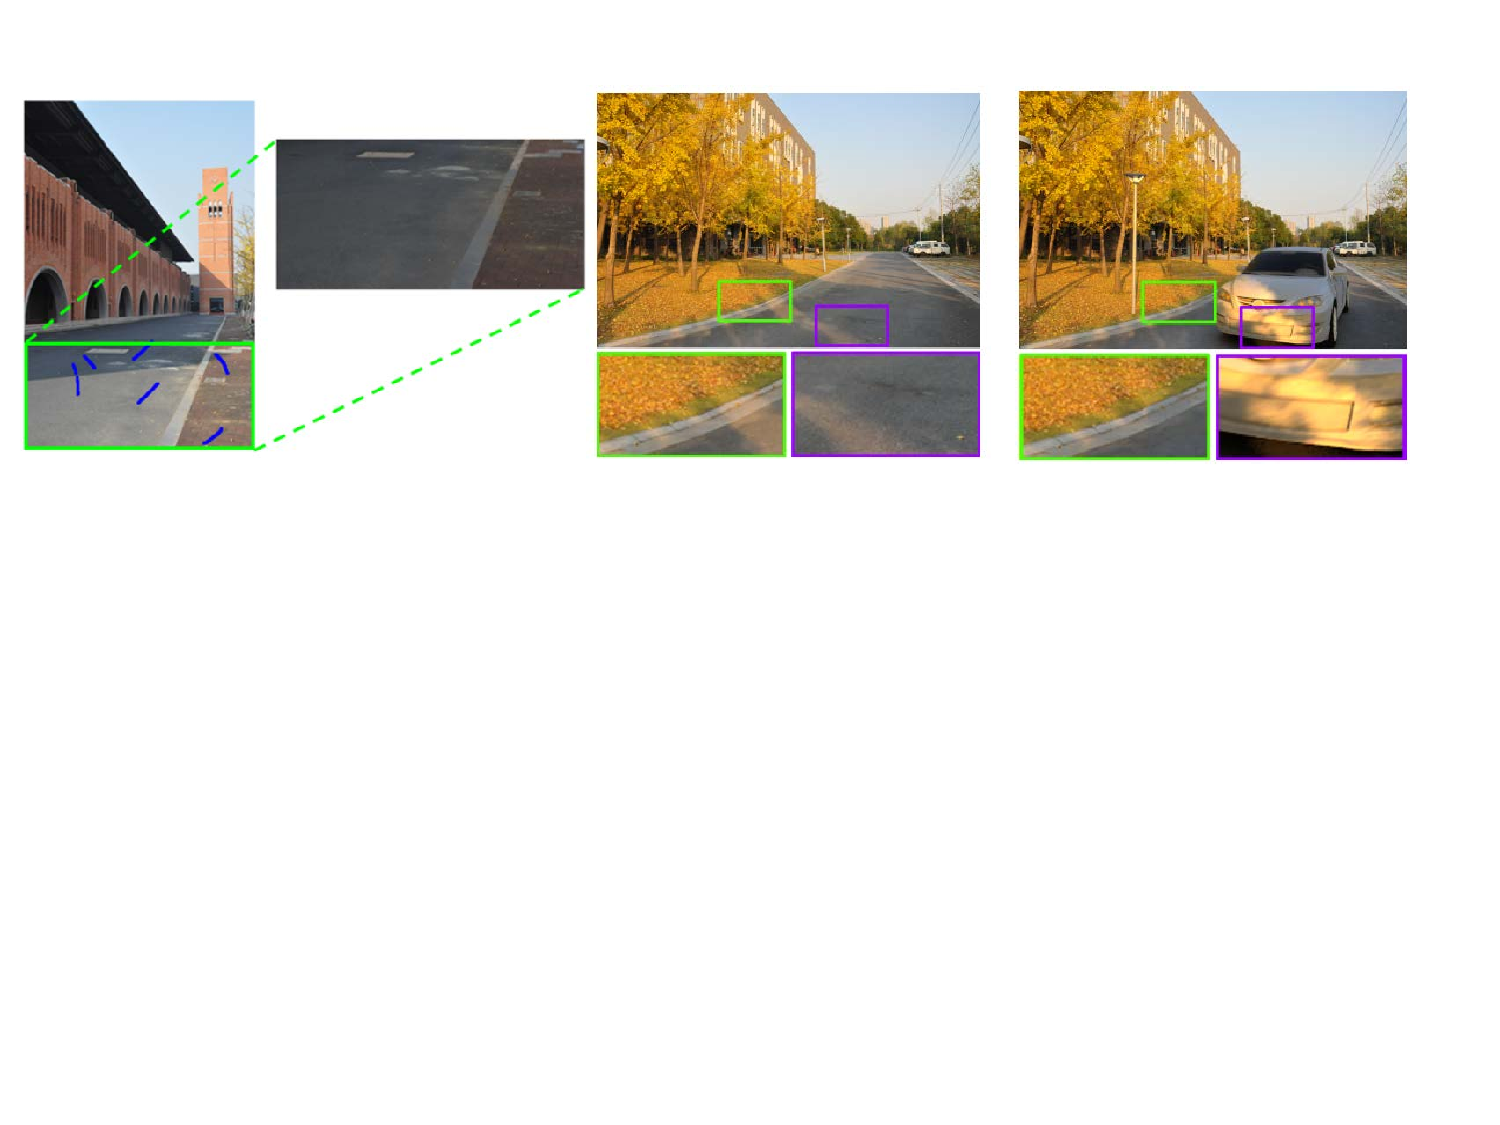
\includegraphics[width=1.0\textwidth]{Img/user-aux.pdf}

    \caption[用户标记辅助估计光照]
    {Xing等人\cite{xing2013lighting}的方法中用户所标记的平面、阴影等参考线,以及最后的图片合成效果}
    
    \label{fig:user-aux}
\end{figure}

这类方法与使用额外信息的方法类似,但这种方法不需要额外的设备去单独拍摄辅助信息。对于用户交互式的应用场景,用户的交互比其它额外的信息更容易获取。不过,使用用户标记信息辅助估计光照也有使用场景限制,需要有用户交互应用时才可以使用这类方法。
\subsection{使用图像分析的方法估计光照}
经过前人多年的工作积累,一些研究者尝试探究仅使用单张图片来进行光照估计,不借助任何额外的辅助信息、特定设备、几何信息等。
Karsch等人\cite{karsch2014automatic}在2014年提出了这样的方法。他们提供了一个用户友好的图像编辑系统。用户将任意的3D虚拟物体拖放置场景后,系统会自动地对其进行渲染。用户后期还可以对其进行再编集。他们的系统是完全自动的,通过一张图片,就可以恢复出综合的三维场景模型(几何、照明、漫反射反照率和相机参数)。为了实现该算法,他们首先从图片中估计出场景的结构信息、深度信息、漫反射反照率,相机参数等信息,然后在SUN360全景数据集\cite{xiao2012recognizing}中查找外观与输入图像相似的全景图,并使用这些全景图中预先分类的光源作为输入图像的光源,获得了较为可靠的光照估计结果。
\cite{chen2014lighting}在估计光照时另辟蹊径,提出了一种新的基于光线和语义的照明模型参数估计方法,该方法利用现有场景理解技术估计出粗糙的场景信息,接着使用标准和语义约束的一组稀疏的小三维曲面进行本征图像分解,最后将得到的粗糙阴影图像视为所选小表面的辐照度。该方法不需要任何预先记录的三维几何图形、反射率、照明采集设备或图像的成像信息,仅使用一张图片作为输入就可以获得较好的结果。

这类方法致力于不使用额外信息,直接从图片中估计场景光照,是解决光照估计问题时的积极探索。但很显然,这类算法非常复杂,难以做到实时,并且每一步都非常依赖上一步的可靠结果。
\subsection{基于深度学习的光照估计方法}
卷积神经网络(CNN)最早由Lecun等人\cite{lecun1998gradient}在1998年提出. 随着计算机显卡性能的提高和超大规模数据集(例如ImageNet\cite{deng2009imagenet},ShapeNet\cite{chang2015shapenet})的建立,深度学习在多个领域成为了一个强力的工具。近年来,为了解决各种类型的问题,卷积神经网络结构层出不穷,例如AlexNet~\cite{krizhevsky2012imagenet}, VGG~\cite{simonyan2014very}, ResNet~\cite{he2016deep}。它们在许多视觉问题中超越了传统方法中取得的非常好的成绩,例如物体检测\cite{girshick2014rich}、图像分类\cite{krizhevsky2012imagenet}、图像分割\cite{ronneberger2015u}等等。近期,卷积神经网络也被应用到了传统的图形学问题中,例如渲染降噪\cite{chaitanya2017interactive}、人脸模拟\cite{karras2017audio}等等,都取得了很好的结果。

近期许多工作尝试使用深度学习解决光照估计问题。和传统方法类似,使用深度学习求解光照估计问题时也会借助一些辅助信息、探测物等。Calian等人\cite{calian2018faces}使用人脸作为光探测物,搭建了神经网络从照片恢复出室外场景的光照。Yi等人\cite{yi2018faces}搭建了一个高光提取神经网络和阴影反照率估计网络,来从人脸照片中恢复出室内外场景的光照信息。
Georgoulis等人\cite{georgoulis2016delight}使用真实反射图作为输入,用两个不同的CNN结构将图片分解为材质变量和光照变量。之后Geogoulis等人\cite{georgoulis2016natural}又尝试利用深度学习从包含多种已知材质的物体图片中恢复出反射图和光照分布。Mandl等人\cite{mandl2017learning}、Weber等人\cite{weber2018learning}也是借用了已知的物体几何恢复出场景光照。虽然这些光照方法和传统方法类似,也借助了一些额外的信息。但通过将传统方法中复杂的算法步骤替换为用深度学习求解,往往能取得更好的结果,这通常得益于大规模的训练数据。
\begin{figure}[!htbp]
    \centering
    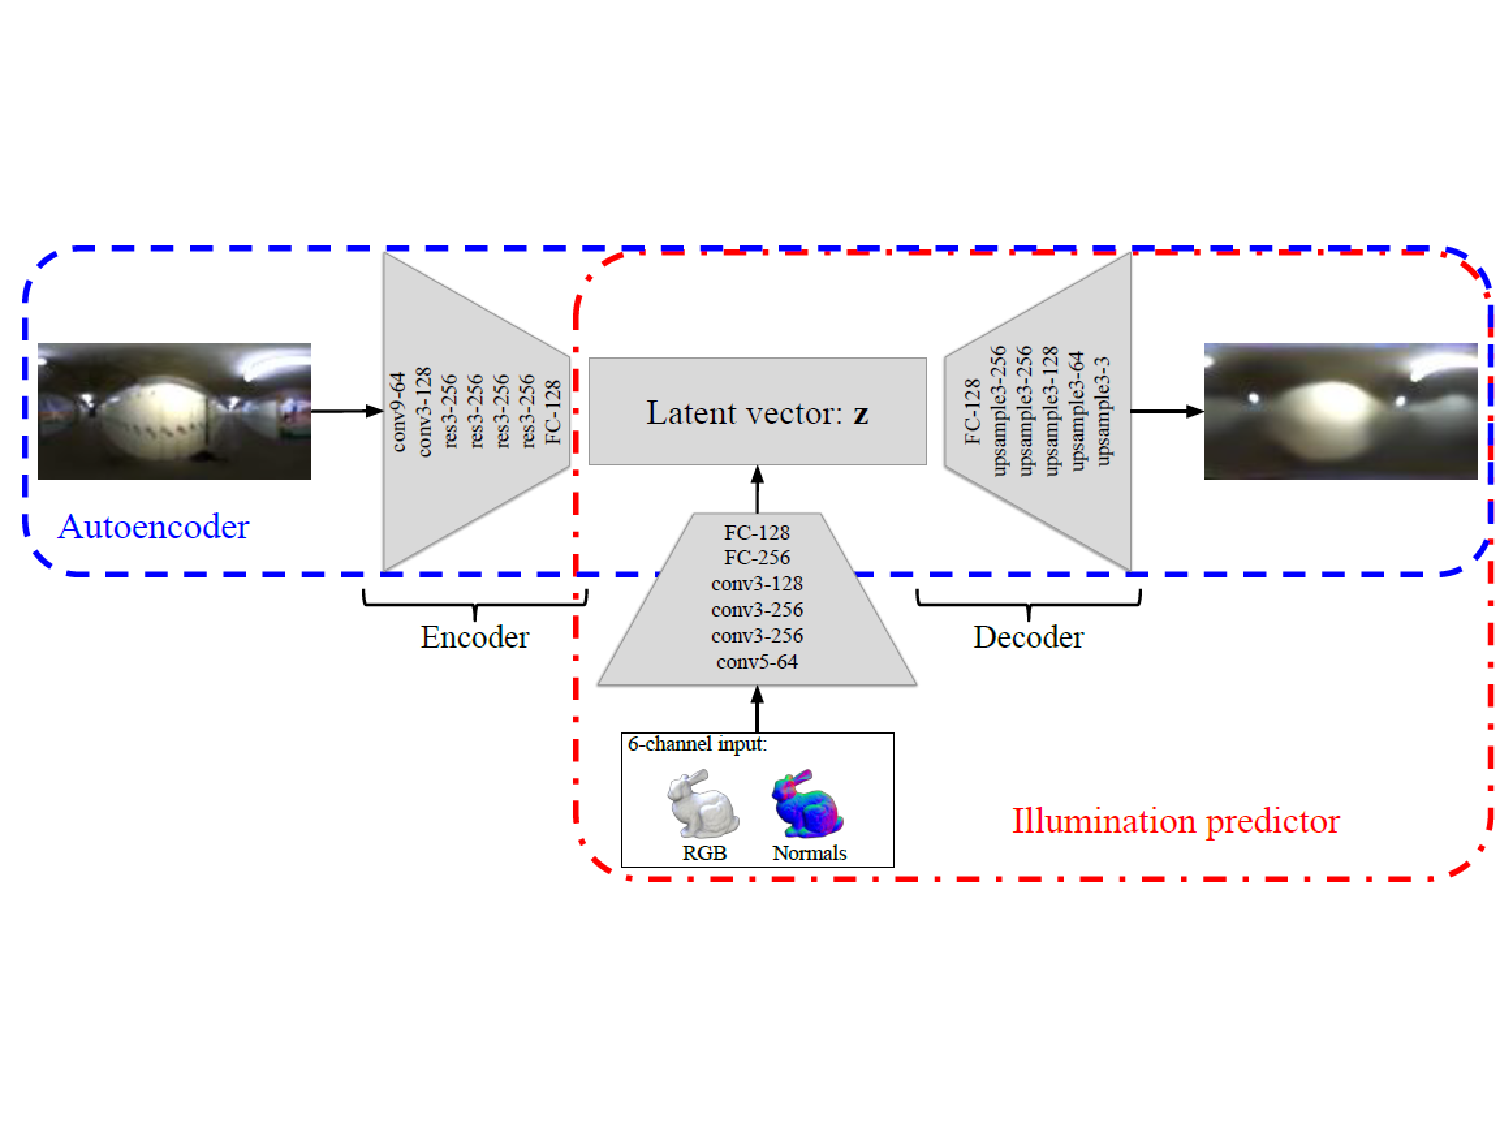
\includegraphics[width=1.0\textwidth]{Img/auto-encoder.pdf}

    \caption[光照的自编码器结构]
    {Weber\cite{weber2018learning}等人结合深度学习工具对光照分布进行编码,该图是其使用的自编码器结构。蓝色边框内为训练自编码器的结构,红色边框内则为训练光照估计的结构。}
        
    \label{fig:auto-encoder}
\end{figure}
使用深度学习求解光照估计问题时,也会使与传统方法中相同的光照表示模型。例如基于物理的Sun-sky模型\cite{hold2017deep}, 球形谐波函数模型\cite{mandl2017learning}等。深度学习在学习输入图像的特征时非常有效,因此Weber等人\cite{weber2018learning}结合深度学习,使用自编码器(auto-encoder)对光照分布进行建模(如图\ref{fig:auto-encoder}),使用卷积神经网络将场景编码为包含少量系数的隐变量,为光照估计问题中光照的表示提供了新的思路。

考虑到CNN强大的学习能力,最近一些方法尝试使用深度学习工具直接从单张图片中恢复整个场景的光照分布。
Holdgeoffroy等人\cite{hold2017deep}搭建了一个深度卷积神经网络从室外图片中恢复出室外场景的参数化光照模型。Gardner等人\cite{gardner2017learning}从室内图片中直接估计HDR全景图像。这两个方法是目前单图片光照估计工作中最先进的方法。
由于HDR全景数据有限,这些方法设计了一个光源探测系统,将大量的低动态范围全景图转化为粗糙的高动态范围全景图用于训练。

在深度学习任务中,训练神经网络需要大规模的高质量数据,但目前来说还没有这样的数据在规模和质量上同时满足要求。用于光照估计问题的数据集由两类,一类是规模较大的低动态范围全景数据集(例如SUN 360\cite{xiao2012recognizing}),这类数据规模较大(数万张),但是低动态范围全景图无法直接应用于光照估计,需要使用特定的算法将其转换为粗糙的、低质量的高动态范围全景图;另一类是规模较小的高动态范围全景数据集(例如Laval Indoor\cite{gardner2017learning},这类数据虽然可以直接应用于光照估计,但是规模较小,难以保证训练的效果。

\section{论文研究内容}
将本文的主要工作内容包括:
\begin{itemize}
    \item 深入调研全景图以及高动态范围全景图的获取步骤、投影方法、存储方式等,使用全景相机和曝光融合算法构建一个用于光照估计、大规模、高质量的HDR全景数据集,并通过实验验证该数据集相对于其它数据集在光照估计问题中的优越性。
    \item 通过详细的实验分析了HDR全景数据集的规模和多样性对于光照估计问题的影响,研究丰富的数据多样性和较大的数据规模是否能够为基于深度学习的光照估计结果带来有效提升。
    \item 分析和验证使用视角相对的图片作为光照估计的输入的可行性。这两张图片可以由相机的前后置摄像头拍摄。使用前后摄像头同时拍摄两张照片不仅不会增加获取图片的步骤,还可以极大地降低光照估计的难度。这对于光照估计在智能设备中的应用来说有着很大的实际意义。
    \item 构建一个基于深度学习的光照估计网络模型,模型应使用两张图片作为输入估计预测出场景的光照分布。并通过实验与state-of-the-art方法的结果进行多项对比。
    \item 对提出的光照估计深度学习模型和损失函数进行十分详尽的实验和分析,对于光照估计网络结构和训练过程中各个模块,设计大量对比实验深入探索使用不同网络结构的特点和对结果的影响,促进了对基于深度学习光照估计的理解。
\end{itemize}